Before we started coding we made a draft of the class diagrams. Throughout the following sprints we kept maintaining and updating the class diagram
draft to make sure that the code and class diagram were in agreement. The class diagram shown and explained below is the final version for our
system.

The class diagram is made in the Unified Modeling Language (UML) to ensure common understanding, when describing the structure of our system.

\begin{figure}[htb]
    \begin{center}
        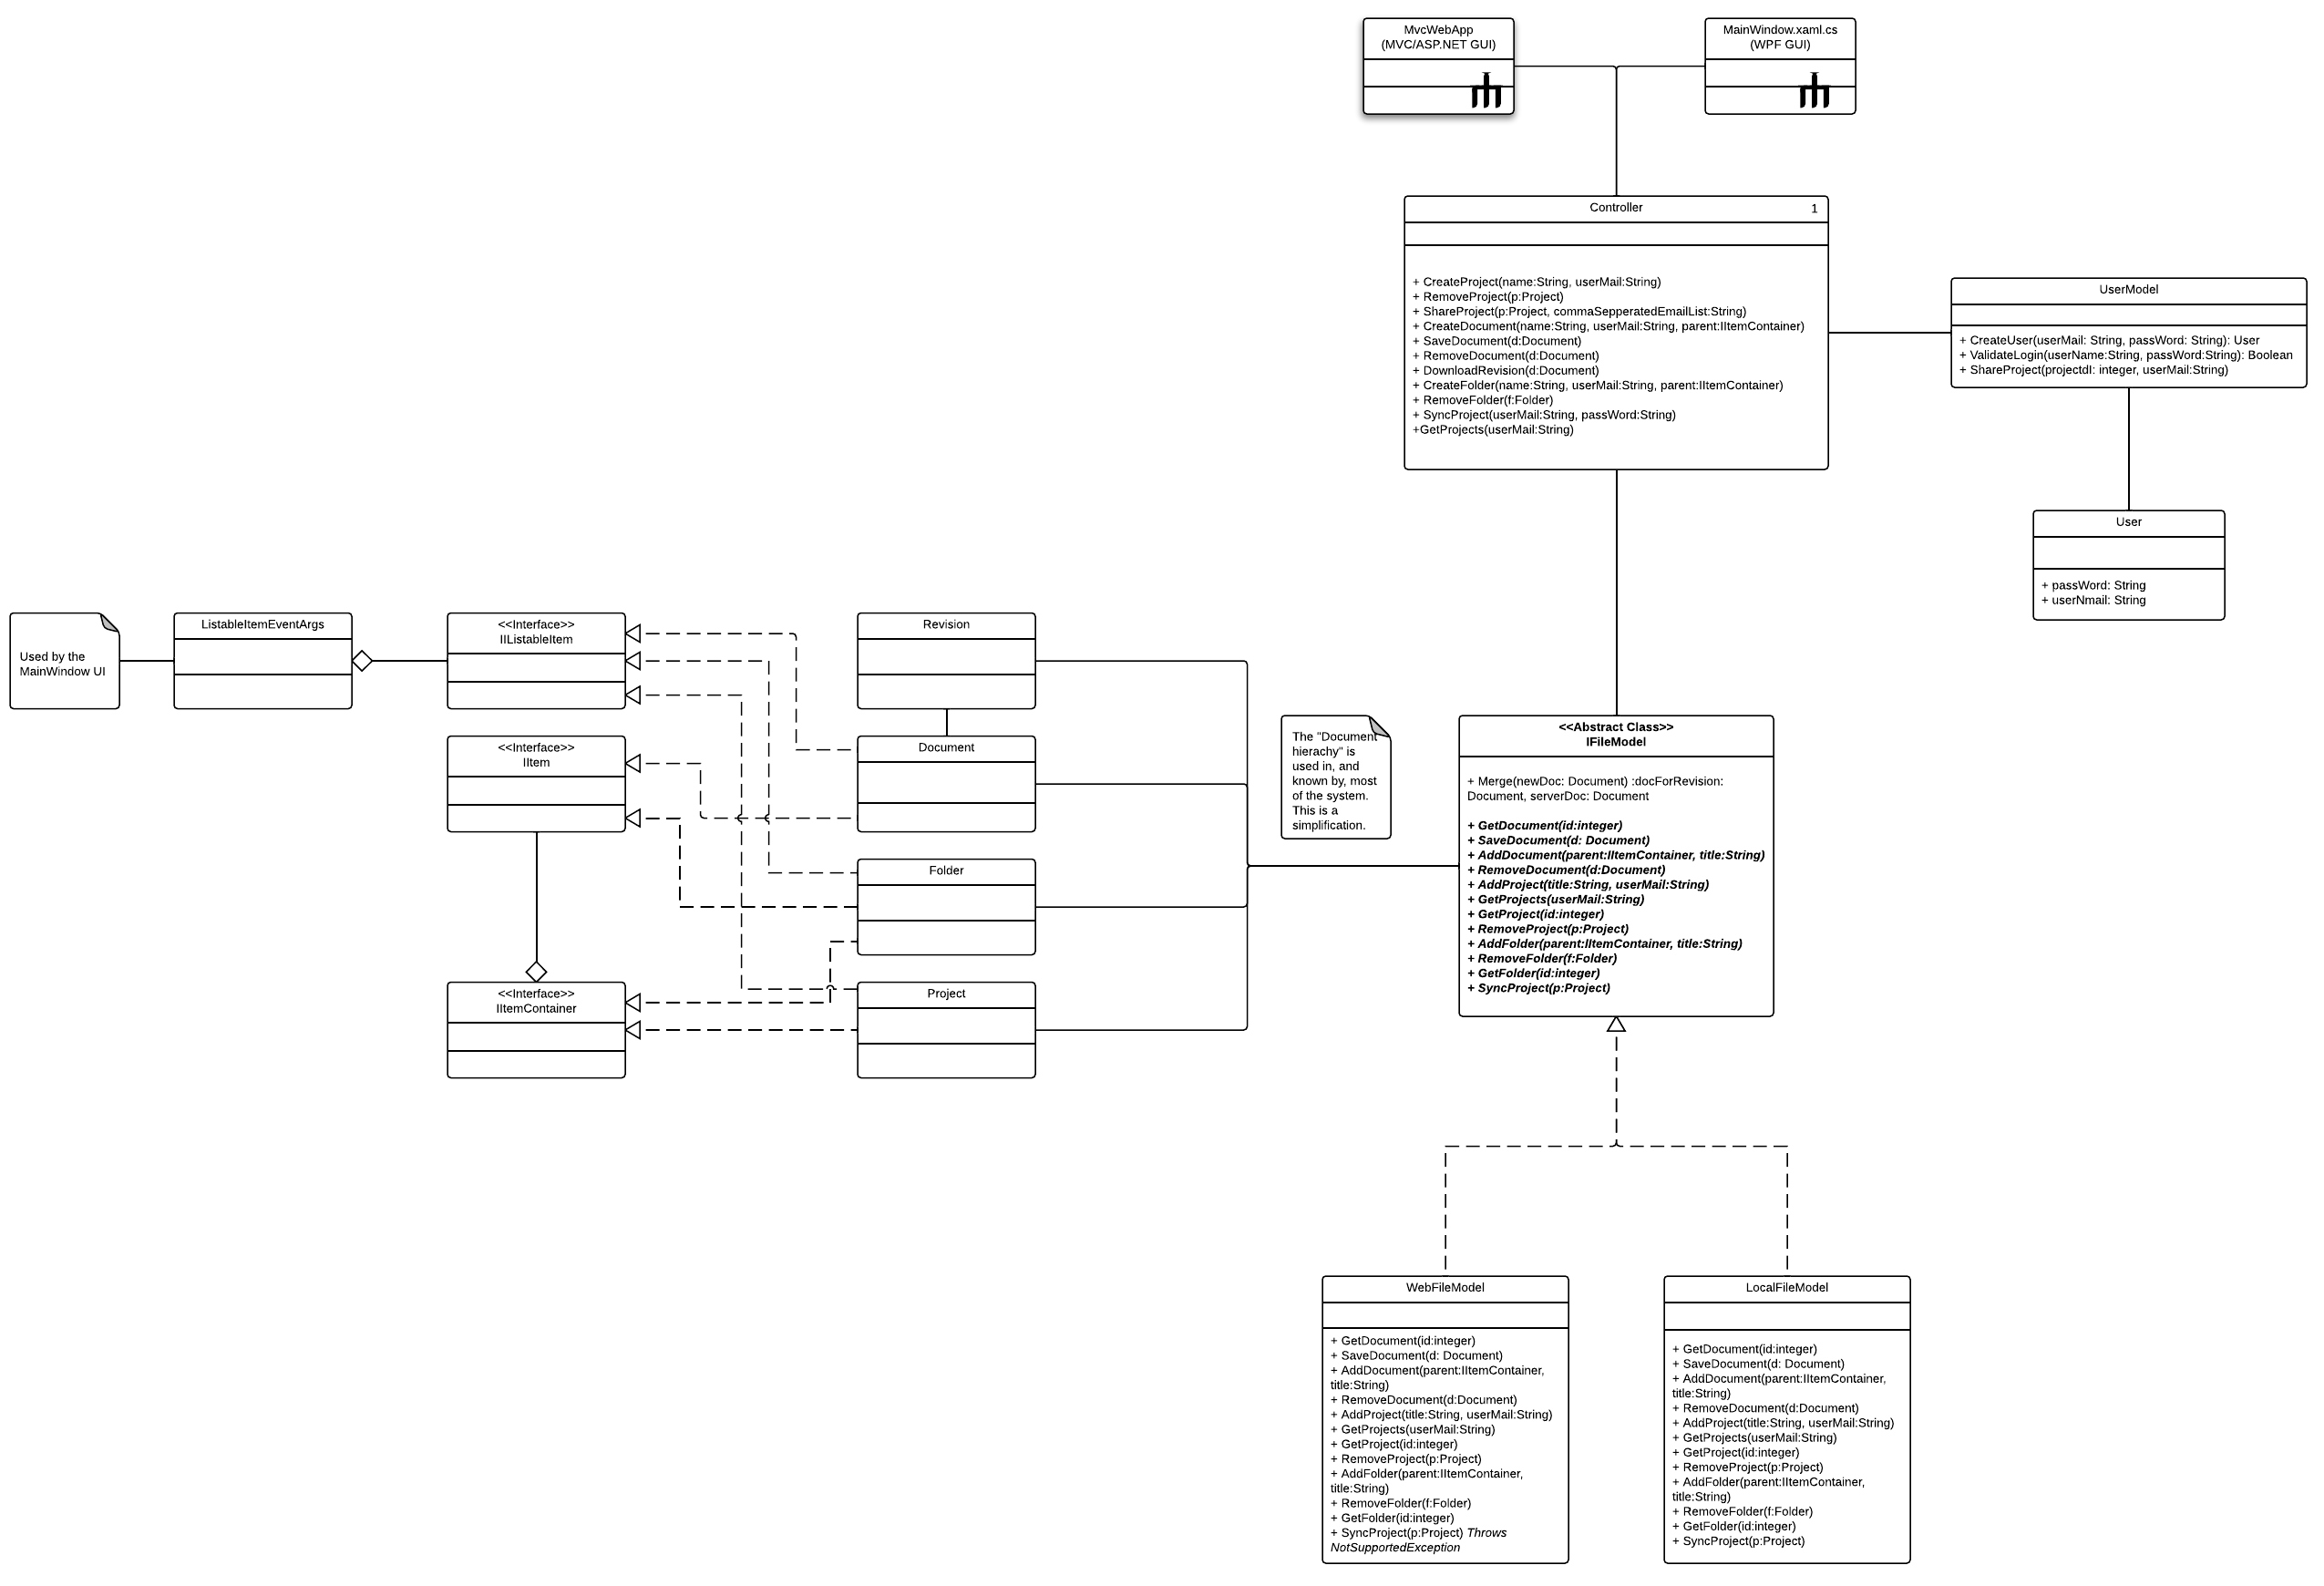
\includegraphics[width=1\textwidth]{Software_design/graphics/mainClassDiagram.png}
        \caption{Overview of the main class diagram for 'Slice of Pie'}
        \label{fig:design-class_diagram}
    \end{center}
\end{figure}

In (Figure~\ref{fig:design-class_diagram}) the most critical and important classes are shown with their most important public methods. 
